\section{Koszt funkcji}\label{chapter:results_cost}

Miarą, która wynika bezpośrednio z czasu działania funkcji oraz rozmiaru jej pamięci jest koszt jej działania.
W ramach badania został on obliczony na bazie średnich czasów procesowania funkcji, co zostało opisane w Rodziale \ref{chapter:cel_i_metodyka_badan}.
W obliczeniach przyjęto 500 wywołań funkcji na sekundę oraz koszt 0.0000166667 USD za GB-sekundę \cite{awsLambdaPricing}.
Wyniki dla poszczególnych metod i rozmiarów pamięci zostały przedstawione na Rysunku \ref{fig:avg_costs}.

\begin{figure}[h]
    \centering
    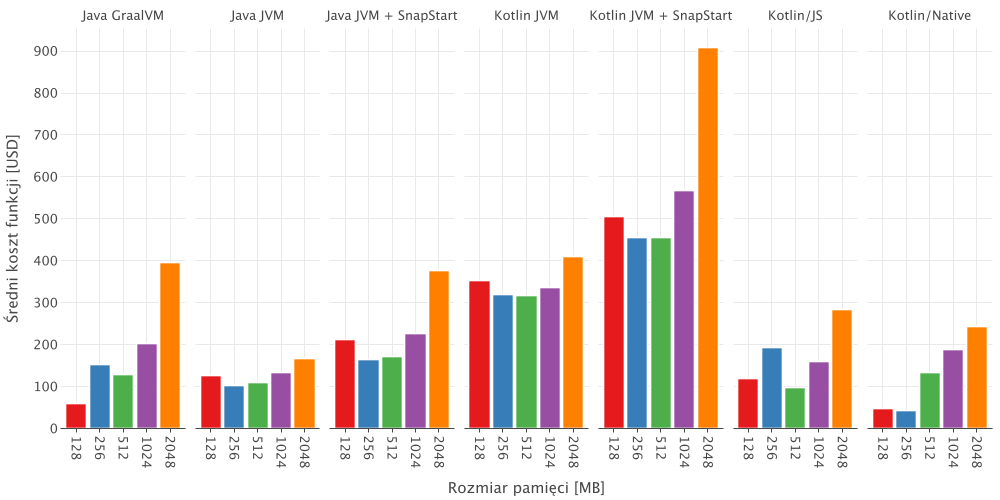
\includegraphics[width=0.95\textwidth]{charts/results/average-cost.png}
    \caption{Średni koszt funkcji w zależności od rozmiaru pamięci [źródło: opracowanie własne]}
    \label{fig:avg_costs}
\end{figure}

Analizując cztery funkcje oparte o JVM można zauważyć, że koszt jest najniższy dla pamięci 256 MB lub 512 MB.
Interesującym faktem jest, że rozmiaru 128 MB koszt działania jest wyższy, co przeczy oczekiwaniom, że koszty maleją wraz z spadkiem wielkości pamięci, niezależnie od jej wartości.
Dla funkcji bez aktywowanej usługi SnapStart koszt dla pamięci 128 MB jest nawet wyższy niż dla wielkości 512 MB.
Podczas aktywnej usługi SnapStart, badane funkcje wykazują znaczny wzrost średnich kosztów wraz z wzrostem pamięci z 1024 MB do 2048 MB.
Sama metoda SnapStart wpływa jednak negatywnie na koszt działania.
Znaczne oddziaływanie rozmiaru pamięci na koszt funkcji jest istotnie widoczny dla Kotlin/JS.
Koszt jest znacznie zróżnicowany, jednak dla pewnych przypadków (pamięć 128 MB i 512 MB) pozostaje on niższy niż w przypadku funkcji Java JVM.

Obie z badanych funkcji natywnych (Java GraalVM, Kotlin/Native) wykazują wzrost kosztów wraz z wzrostem rozmiaru pamięci.
Dla każdego rozmiaru pamięci oprócz 128 MB, koszty funkcji Java GraalVM są wyższe niż dla analogicznej funkcji Java JVM.
Widoczny jest także znaczny wzrost kosztów dla pamięci 2048 MB, podobnie jak w przypadku usługi SnapStart.
W przypadku użycia Kotlin/Native i pamięci 128 MB lub 256 MB możliwe jest osiągnięcie najniższych kosztów działanio (odpowiednio 48 i 43 USD).
Dla większych rozmiarów najlepsze wyniki zostały osiągnięte przez Kotlin/JS (rozmiary 512 MB) i Java JVM (rozmiary 1024 MB i 2048 MB).
